% Work-MAT | 2. rocnik | pripravovana hodina 54
% Návaznost: uživatelské připravy.zip (hodiny 01–20), autorská učebnice na GitHubu.
% Realisticky.cz: didaktická inspirace v posloupnosti a typech úloh; zadání jsou vlastní.
\documentclass[11pt,a4paper]{article}
\input{../../sablony/pripravy/priprava.sty}
\usepackage{tikz}
\nastavPripravu{2. ročník}{Goniometrické funkce}{54}{Určování úhlů z hodnot}
\begin{document}
\blok{Motivace a návaznost}
Dnes pracujeme obráceně: z hodnoty sin nebo cos hledáme všechny přípustné úhly v jedné otáčce. Žáci musí využít souměrnost na kružnici.
\poznamka{Orientační nabídka pro 45--55 minut: krátké zopakování a motivace, nový výklad, tři společné vzorové úlohy, samostatná práce. Vyber podle tempa třídy; zbývající zadání slouží jako rezerva.}
\blok{Výklad}
Pro $\sin x=c$ bývají v intervalu $[0;2\pi)$ dvě řešení; pro extrémní hodnoty $c=\pm1$ právě jedno.
\begin{center}
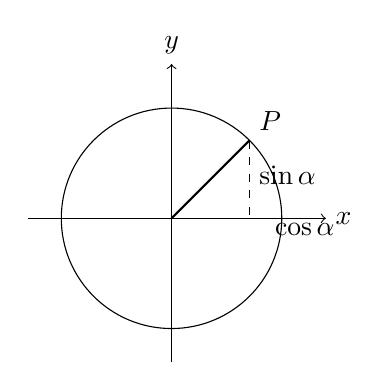
\begin{tikzpicture}[scale=1.4]
\draw[->] (-1.3,0)--(1.4,0) node[right] {$x$};
\draw[->] (0,-1.3)--(0,1.4) node[above] {$y$};
\draw (0,0) circle (1);
\draw[thick] (0,0)--(0.7071,0.7071);
\draw[dashed] (0.7071,0.7071)--(0.7071,0);
\node[above right] at (0.7071,0.7071) {$P$};
\node[below right] at (0.85,0.04) {$\cos\alpha$};
\node[right] at (0.7071,0.39) {$\sin\alpha$};
\end{tikzpicture}
\end{center}
\blok{Společné příklady}
\begin{prikladReseniBox}[title={Příklad 1}]
Vyřeš, resp. urči: $\sin x=\frac{\sqrt3}{2},\quad x\in[0;2\pi)$.
\tcblower
\[\begin{aligned}x=\frac{\pi}{3}\;\lor\;x=\frac{2\pi}{3}\end{aligned}\]
\end{prikladReseniBox}
\begin{prikladReseniBox}[title={Příklad 2}]
Vyřeš, resp. urči: $\cos x=0,\quad x\in[0;2\pi)$.
\tcblower
\[\begin{aligned}x=\frac{\pi}{2}\;\lor\;x=\frac{3\pi}{2}\end{aligned}\]
\end{prikladReseniBox}
\poznamka{Uveď jednu hodnotu v každém příslušném kvadrantu. Na závěr odliš výsledek v jedné otočce od všech řešení na $\mathbb R$.}
\blok{Samostatné procvičování}
\begin{zadaniReseniBox}[title={Samostatná práce 1}]
\begin{enumerate}[label=\alph*)]
\item $\sin45^\circ$.
\item $\cos45^\circ$.
\item $\sin150^\circ$.
\item $\cos150^\circ$.
\item $\operatorname{tg}135^\circ$.
\item $\operatorname{cotg}45^\circ$.
\end{enumerate}
\tcblower
\begin{enumerate}[label=\alph*)]
\item $\frac{\sqrt2}{2}$.
\item $\frac{\sqrt2}{2}$.
\item $\frac{1}{2}$.
\item $-\frac{\sqrt3}{2}$.
\item $-1$.
\item $1$.
\end{enumerate}
\end{zadaniReseniBox}
\blok{Dobrovolné rozšíření}
\begin{zadaniReseniBox}[title={Rozšíření 1}]
\begin{enumerate}[label=\alph*)]
\item Navrhni obdobnou úlohu s jiným úhlem a zkontroluj výsledek graficky..
\end{enumerate}
\tcblower
\begin{enumerate}[label=\alph*)]
\item $Srovnej s jednotkovou kružnicí nebo grafem.$.
\end{enumerate}
\end{zadaniReseniBox}
\blok{Úkol na doma}
Každou hodnotu zdůvodni náčrtkem jednotkové kružnice nebo orientovaným úhlem; u přesných hodnot neuváděj jen desetinné aproximace.
\begin{zadaniReseniBox}[title={Domácí úkol}]
\begin{enumerate}[label=\alph*)]
\item $\sin210^\circ$.
\item $\cos240^\circ$.
\item $\operatorname{tg}60^\circ$.
\item $\operatorname{cotg}60^\circ$.
\item $\sin330^\circ$.
\item $\cos300^\circ$.
\item $\sin270^\circ$.
\item $\cos180^\circ$.
\end{enumerate}
\tcblower
\begin{enumerate}[label=\alph*)]
\item $-\frac{1}{2}$.
\item $-\frac{1}{2}$.
\item $\sqrt3$.
\item $\frac{\sqrt3}{3}$.
\item $-\frac{1}{2}$.
\item $\frac{1}{2}$.
\item $-1$.
\item $-1$.
\end{enumerate}
\end{zadaniReseniBox}
\poznamka{Domácí úkol obsahuje 8 položek; předpokládaná domácí práce přibližně 15--30 minut. Po větších blocích jsou vědomě promíchané dříve probrané typy.}
\end{document}
